\documentclass[]{exam}
\title{Computer Architecture - TE2031}
\date{February - June 2020}


\newif\ifanswers
%\answerstrue % comment out to hide answers


% Begin document
\begin{document}

\section*{Ideas for exam questions}

\begin{enumerate}
% ====================
\item Exercise A.23 and A.24 Weste.
\item Scaled memory addressing could be used for
a) Accessing page memory
\item Provide a waveform diagram with an input D for both \ac{FF} and latch. The student must provide outputs Q for both devices. Moreover, Make input D to change during and after the active level of the latch. Extra difficulty, make both devices active low using their schematic.

\ifanswers\\
\alertred{5/15}\\
Both latches and \acp{FF} are sensitive to a clock signal. However, \acp{FF} are edge-sensitive devices,\ie rising and falling edges, whereas latches are level-sensitive devices. 
\begin{figure}[!h]
\centering
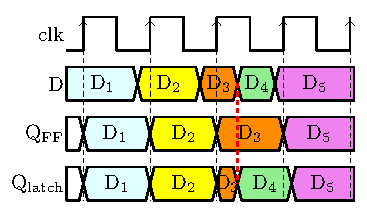
\includegraphics[scale=1]{dff_latch}
\label{Figure:FF_latch}
\caption{Difference between \acp{FF} and latches.}
\end{figure}
\fi

% ====================
%\item What's the difference between a half-adder and a full-adder?
%\ifanswers\\
%\alertred{13/21}\\
%A full-adder has a carry input.
%\fi

% ====================
\item Provide the student with a block diagram of both Mealy and Moore machines. Make the student identify each of them.
\ifanswers\\
\alertred{0/16}\\
The output of a Moore machine depends \textbf{\textcolor{blue}{only}} on the current state of the machine, whereas a Mealey output depends on both the current state and the inputs of the machine.  
\fi

% ====================
\item How would you obtain the number of bits $n$ in order to represent the decimal number $x$, where $x>0$?

\ifanswers\\
\alertred{18/24}
$\ceil{log_{2}(938)} = 10$
\fi

\item Provide the student with a list of RISC and CISC characteristics. Ask the student to put the characteristics in each RISC/CISC column?

\item Which RISC or CISC makes a more efficient RAM usage? A: CISC due to a more efficient encoding.

\ifanswers\\
\alertred{18/24}
$\ceil{log_{2}(938)} = 10$
\fi
% ====================
%\item What's the difference between asynchronous and synchronous reset?
%\ifanswers\\
%\alertred{13/19}\\
%An asynchronous reset does not depend on the clock signal. As a result of this, all \ac{FF} connected to an asynchronous reset would reset their value when the reset signal is asserted. On the other hand, synchronous resets must wait for an active clock edge in order to trigger the reset function. 
%\fi

% ====================
\item In \SV, what's the difference between blocking and non-blocking assignments?
\ifanswers\\
\alertred{0/5}\\
\alertred{Blocking} assignments, \alertred{=}, are used to model \alertred{combinational} logic.
The name `blocking' comes from the idea that one assignment \emph{blocks} the subsequent assignments, \ie, the code is executed \emph{sequentially}.

\alertblue{Non-blocking} assignments, \alertblue{\textless{}=}, are used to model \alertblue{sequential} logic.
The name `non-blocking' comes from the idea that all assignments in a process are evaluated at the same time, \ie, the code is executed in \emph{parallel}.
\fi

% ====================
\item Using the hardware description language of your choice (Verilog, \SV or VHDL), write down the code for a D-type flip-flop with asynchronous reset.
\ifanswers\\
\alertred{3/7}\\
\lstset{
        basicstyle=\small,
        xleftmargin=.03\textwidth, 
        caption=Asynchronous reset D-type \ac{FF} \SV module., 
        label=listing:DFF_SV
        }
\lstinputlisting{../SystemVerilog/dff_async_reset/dff_async_reset.sv}
\fi

% ====================
\item In your own words, briefly describe the design flow of a digital integrated circuit.
\ifanswers
\alertred{1/4}\\
\fi

% ====================
\item Represent the signed decimal number -1 using 4-bits two's complement. 
\ifanswers\\
\alertred{13/19}\\
\code{1111}
\fi

% ====================
\item What's the dynamic range $d$ (minimum and maximum decimal values) that may be represented using 8-bits in two's complement?
\ifanswers\\
\alertred{3/14}\\
\begin{center}
$ d \in [-2^{n-1}, 2^{n-1}-1]$\\
$ d \in [-2^{7}, 2^{7}-1]$\\
$ d \in [-128,127]$\\
\end{center}
\fi

% ====================
\item In digital arithmetic, what is overflow?
\ifanswers\\
\alertred{16/17}\\
Overflow occurs when the result of an arithmetic operation can not be represented with the available numbers of bits.
\fi

% ====================
\item Design a 2-input AND gate using a multiplexer.
\ifanswers
\alertred{4/11}\\
\begin{figure}[!h]
\centering
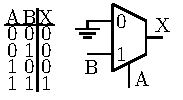
\includegraphics[scale=1.8]{AND2_MUX}
\label{Figure:AND2_MUX}
\caption{AND2 gate from MUX.}
\end{figure}
\fi

% ====================
\item What's the difference between RAM and ROM memories?
\ifanswers\\
\alertred{18/20}\\
RAMs are read/write volatile memories. Once their power supply is switched off, their will lose their contents. By contrast, ROMs are read-only non-volatile memories, \ie, their contents will remain even after switching their power supply off.
\fi

% ====================
\item Convert the 16-bit hexadecimal number C4E7 to binary.
\ifanswers\\
\alertred{15/20}\\
\code{1100 0100 1110 0111}
\fi

% ====================
\item Convert the fractional binary number 10111111.1001 to decimal.
\ifanswers\\
\alertred{3/16}\\
\begin{equation*}
  \begin{array}{rl}
  10111111.1001_{b} = & ~~~ 1\times2^{7}  \\
                      & + 0\times2^{6}  \\
                      & + 1\times2^{5}  \\
                      & + 1\times2^{4}  \\
                      & + 1\times2^{3}  \\
                      & + 1\times2^{2}  \\
                      & + 1\times2^{1}  \\
                      & + 1\times2^{0}  \\
                      & + 1\times2^{-1}  \\
                      & + 0\times2^{-2}  \\
                      & + 0\times2^{-3}  \\
                      & + 1\times2^{-4} \\
                    = & 191.5625
  \end{array}
\end{equation*}
\fi

% ====================
\item Using Sum-of-Products, derive the Boolean expression for X from the following truth table. A, B and C are inputs, X is the output.\\
\ifanswers
\alertred{13/18}\\
\begin{table}[!h]
\centering
\begin{tabular}{ccc|cc}
A & B & C & X & \\\hline
0 & 0 & 0 & 0 & \\
0 & 0 & 1 & 0 & \\
0 & 1 & 0 & 1 & $\overline{A}~B~\overline{C}$\\
0 & 1 & 1 & 1 & $\overline{A}~B~C$\\
1 & 0 & 0 & 1 & $A~\overline{B}~\overline{C}$\\
1 & 0 & 1 & 0 & \\
1 & 1 & 0 & 1 & $A~B~\overline{C}$\\
1 & 1 & 1 & 1 & $A~B~C$\\
\end{tabular}
\end{table}
\fi

% ====================
\item Use a Karnaugh map in order to obtain a Boolean expression for X from question 16.
\ifanswers
\alertred{11/15}\\
\begin{figure}[!h]
\centering
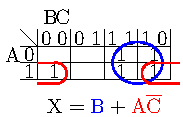
\includegraphics[scale=1.8]{karnaugh_map}
\label{Figure:karnaugh_map}
\end{figure}
\fi

% ====================
\item What is the difference between a \ac{FPGA} and an \ac{ASIC}?
\ifanswers\\
\alertred{19/19}\\
The main difference is that \acp{FPGA} are programmable devices, which means their hardware can be configured according the user's need. By contrast, the hardware in an \ac{ASIC} can't be configured or modified after its fabrication.
\fi

% ====================
\item Write down the truth table of a JK flip-flop.
\ifanswers\\
\alertred{0/1}
\begin{table}[!ht]
\centering
\begin{tabular}{cc|c}
J & K & Q \\\hline
0 & 0 & $\mathrm{Q^{-}}$ \\
0 & 1 & 0 \\
1 & 0 & 1 \\
1 & 1 & $\mathrm{\overline{Q^{-}}}$
\end{tabular}
\end{table}
\fi

\end{enumerate}
\end{document}
